\chapter{Software implementation}
%Can put pseudocode in for main steps
%put the details of the examples in results and analysis chapter

\section{Data simulation}\label{sec:sim}
\subsection{Design objectives}
%Pr 1 St 1
%Review primary design objectives
%The major requirements which the objective places on architechure: variability + major corruption classes + framework for implementing signal corruptions  
Our primary aim is to test and research mm-VLBI calibration, imaging and parameter estimation algorithms/strategies through the construction of a synthetic data simulation framework. To address the many questions within the wide scope of this objective, one must be able to setup and run a diversity of experiments within the simulation framework. This places definite constraints on the software architechure. In particular, the framework should 
\begin{itemize}
 \item enable the implementation of all relevant classes of signal corruption within a formalism which ensures consistency with the causal signal transmission chain,
 
 \item be compatible with time-variable GRMHD source models which are to be used as inputs,
 
 \item enable the construction and execution of arbitrary observations,
 
 \item be organised in modularised structure so that it is flexible, extendable and could be incorporated by other interferometric algorithms e.g. a calibration or parameter estimation algorithm.
\end{itemize}

\subsection{Architechure and Workflow}
%Pr 1 st 2
%Intro and plan
In this section, we will review how the architechural design and workflow of the simulator architechure has been designed to meet the above objectives. To fulfill the first objective, we try to cast signal corruptions in the RIME (see section~\ref{sec:RIME}) formalism, and where this is not possible, to fit those particular signal corruptions into the casually correct position in the signal transmission chain. The implementation of each signal corruption is described in the following subsections. The remaining objectives fall into the realm of software design and will be discussed in this subsection.


%Language and data format choice
We have chosen to write the simulator using the \textsc{Python} language. \textsc{Python} is a general purpose language, is geared towards readability, and is well supported by a comprehensive library and wide user base (including astronomers). Specifically \textsc{Python} interfaces well with a modern interferometric toolbox, {\sc MeqTrees}, as well as our data formats of choice: {\sc fits} for image cubes and the {\sc measurement set}\footnote{https://casa.nrao.edu/Memos/229.html} (MS) for visibilities. Although the higher level functionality is written in \textsc{Python}, the bulk of the computational load (MS and visibility generation) is called through lower level programs, which are written in the faster {\sc C++} language. 
The {\sc measurement set} (MS) is data format of choice as it is directly accessible via the {\sc pyrap} library and is the format of choice for {\sc MeqTrees} which is used for computing the RIME. Although in the mm-VLBI subfield other data formats are currently still more popular than the MS i.e. {\sc UVFITS} and/or {\sc HOPS}, with the completion of ALMA, the MS format will inevitably become the next generator data format and already is used at the Joint Institute for VLBI in Europe (JIVE). 


%Conceptual workflow - What are the essentials ins, outs and calculations 

%workflow fig

A conceptual flow diagram of a {\sc MeqSilhouette} simulation pipeline is shown in Fig.~\ref{flow}. The framework is not restricted to this sequence of operations and allows for the exact pipeline to be quite general. This flexibility is made possible through the use of \emph{Object-Orientation}, which will be elaborated on later.

\begin{figure*}
\begin{center}
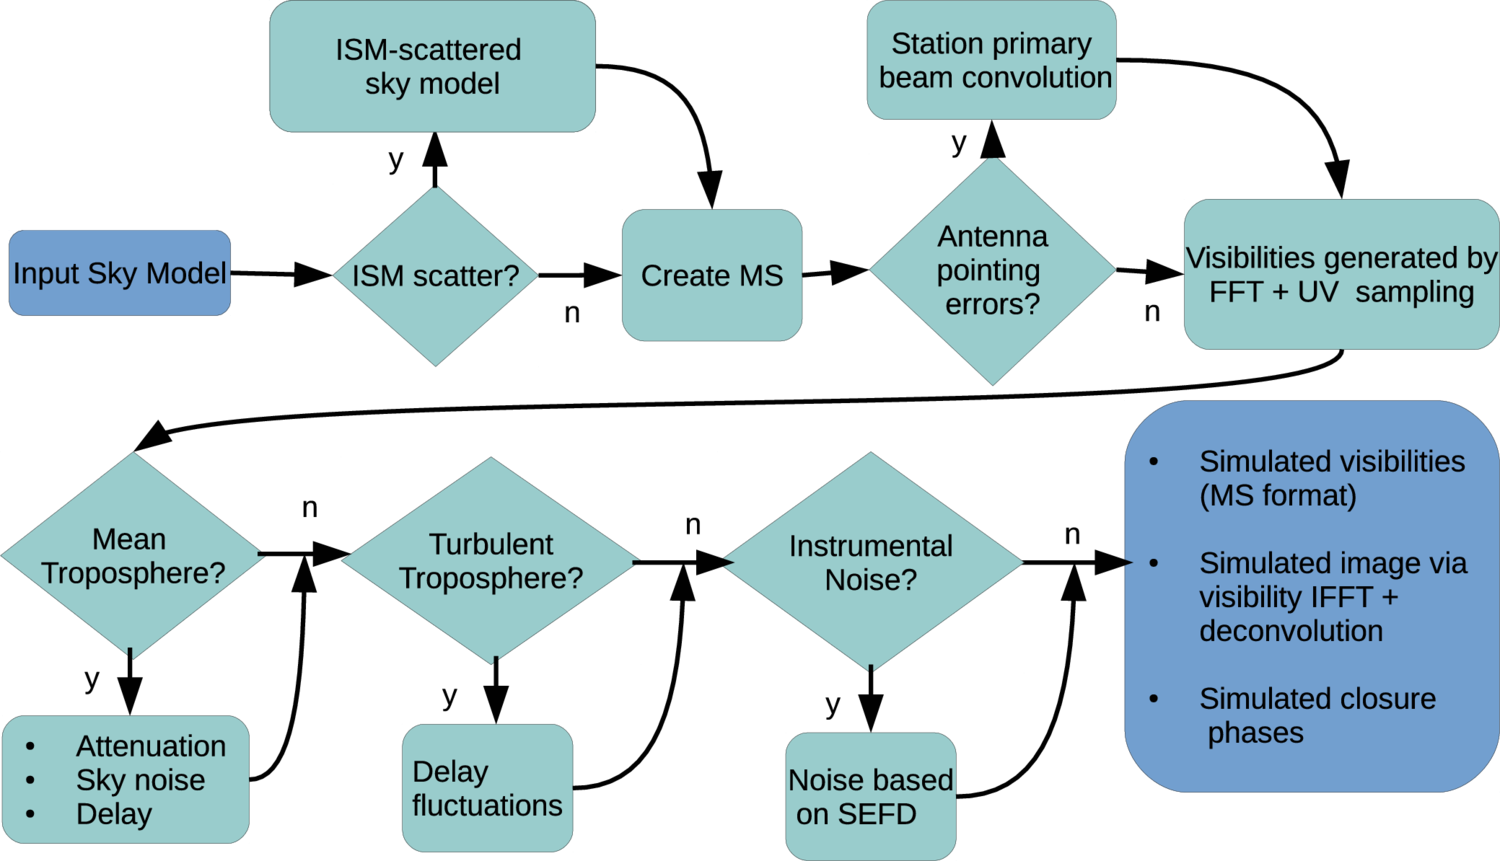
\includegraphics[width=\columnwidth]{Images/flow_full}
\caption{Flow diagram showing basic sequence of the \textsc{MeqSilhouette} simulation pipeline. The sky model could include (a) a time-ordered list of {\sc fits} images or (b) parametric source model consisting of Gaussians or point sources. The details of the station information, observation strategy, tropospheric and ISM conditions are specified in a user-defined input configuration file. The pipeline is flexible, allowing any additional, arbitrary Jones matrices to be incorporated. Further details in text.\label{flow}%
}
\end{center}
\end{figure*}


%Work flow 1 : Inputs & driver script 
At highest level of the framework is the driver script and parameter dictionary. The driver script determines the major sequence of steps in the pipeline whereas the parameter dictionary specifies all parameters needed by the pipeline to determine the particular observation configuration (array, frequency, bandwidth, start time, etc), which signal corruption implementation should be employed and where the sky model is located. The sky model is typically a time-ordered list of {\sc fits} images, where each image represents the source total intensity\footnote{Later versions of {\sc MeqSilhouette} will enable the full Stokes cubes as input.} over a time interval $\Delta t_{\rm src} = t_{\rm obs}/N_{\rm src}$, where $t_{\rm obs}$ is the observation length and $N_{\rm src}$ is the number of source images.


%ms creation 
The first major step in the pipeline is to create the MS. This is performed using the {\sc simms}\footnote{https://github.com/radio-astro/simms} tool. {\sc simms} provides an easy to use interface to construct general MS, given an appropriate antenna table. This includes multiple scans, bands and channels. 



 
 The RIME is evaluated using the MeqTrees : turbo-sim script which visibilities are calculated through evaluation of the Fourier Transform at each UVW coordinate in the dataset, the time and frequency resolution of which is specified by the user.
 
 The primary outputs of the pipeline are an interferometric dataset in {\sc measurement set} format along with the closure phases and uncertainties and a dirty and/or deconvolved image (or spectral cube if desired). 







%Work flow 2 : Calculation and & back end & object orientation
Calculation is object oriented, we have should to create several classes containing Measurement Set and FITS file. The classes are separated as a way of modularisation, separating different level tasks. Makes it easier to debug.

First class is \emph{SimpleMS} which contains only the original measurement set and derivative quantities e.g. calculated station elevations and closure phases. This class serves to make the often used attributes and functions associated with the basic MS easy to access. A key feature of SimpleMS is it specifies a function which is the only way that we have allowed data to be saved into the measurement set (aside from the meqtrees sim). 

The second MS-related class is TropMS which handles all troposphere and thermal noise related corruptions. This class is a child of SimpleMS, hence it has all the attributes and functions of SimpleMS. It also has also the functions and attributes related to the tropospheric corruption - mostly taken from the station information input file.

The third MS-related class is the SimCoordinator class, a child of the TropMS class. SimCoordinator is designed to make various simulations very easy to construct and run. SimCoordinator is set-up and called in the driver script. Along with the functionality and attributes of its parents, SimCoordinator also knows about the input source model and has functionality of the MeqTrees and ISM scattering simulation scripts. Once constructed, SimCoordinator can run ISM scatter, interferometric simulations, tropospheric and instrumental corruptions, thereby presents high level functionality to the user.


%Work flow 3 : Outputs and Data products


The primary outputs of the pipeline are an interferometric dataset in {\sc measurement set} format along with the closure phases and uncertainties and a dirty and/or deconvolved image cube. The modular structure of the pipeline allows for multiple imaging and deconvolution algorithms to be employed. 



\subsection{ScatterBrane}
%Pr 1 St 2
%link back to theory
%Implementation in ScatterBrane : Python, the key algorithmic steps
%Integration of Scatterbrane




\subsection{Atmospheric corruption simulator}
%Pr 1 St 2
%Implementation details of ATM:numerical integration, inputs, outputs, tests, previous use cases
%average/turbulent split

%the turbulent scattering model



\subsection{Pointing error simulator}
%Pr 1 St 2
%The pointing implementation in MeqTrees, WSRT beams, approximating the LMT error
\subsection{RODRIGUES interface}
%Pr 3 St 3
For community use, we host the online, RODRIGUES, interface, found at http://rodrigues.meqtrees.net/. Each of the components of the simulator run in Docker containers. **Looks like the infrustructure is going to change, re: discussions with Gijs and Sphe, so going to wait before writing this.

\section{Parameter estimation}
%Leave for now
